
%%--------------------------------------------------
%% Halliday: Fundamentals of Physics
%%--------------------------------------------------


%% Chapter 06: Force and Motion--II
%%--------------------------------------------------


%% Learning Objectives
%%--------------------------------------------------

%% 6.01: Distinguish between friction in a static situation and a kinetic situation.
%% 6.02: Determine direction and magnitude of a frictional force.
%% 6.03: For objects on horizontal, vertical, or inclined planes in situations involving friction, draw free-body diagrams and apply Newton’s second law.


%% Halliday Multiple Choice Questions
%%--------------------------------------------------
\element{halliday-mc}{
\begin{questionmult}{halliday-ch06-q01}
    A brick slides on a horizontal surface. 
    Which of the following will increase the magnitude of the frictional force on it?
    \begin{choices}
      \correctchoice{Putting a second brick on top}
        \wrongchoice{Decreasing the surface area of contact}
        \wrongchoice{Increasing the surface area of contact}
        \wrongchoice{Decreasing the mass of the brick}
        %\wrongchoice{None of the above}
    \end{choices}
\end{questionmult}
}

\element{halliday-mc}{
\begin{questionmult}{halliday-ch06-q02}
    The coefficient of kinetic friction:
    \begin{choices}
        \wrongchoice{is in the direction of the frictional force}
        \wrongchoice{is in the direction of the normal force}
        \wrongchoice{is the ratio of force to area}
        \wrongchoice{can have units of newtons}
      %\correctchoice{is none of the above}
    \end{choices}
\end{questionmult}
}

\element{halliday-mc}{
\begin{question}{halliday-ch06-q03}
    When the brakes of an automobile are applied,
        the road exerts the greatest retarding force:
    \begin{choices}
        \wrongchoice{while the wheels are sliding}
      \correctchoice{just before the wheels start to slide}
        \wrongchoice{when the automobile is going fastest}
        \wrongchoice{when the acceleration is least}
        \wrongchoice{at the instant when the speed begins to change}
    \end{choices}
\end{question}
}

\element{halliday-mc}{
\begin{question}{halliday-ch06-q04}
    A forward horizontal force of \SI{12}{\newton} is used to pull a \SI{240}{\newton} crate at constant velocity across a horizontal floor. 
    The coefficient of friction is:
    \begin{multicols}{3}
    \begin{choices}
        \wrongchoice{\num{0.5}}
      \correctchoice{\num{0.05}}
        \wrongchoice{\num{2}}
        \wrongchoice{\num{0.2}}
        \wrongchoice{\num{20}}
    \end{choices}
    \end{multicols}
\end{question}
}

\element{halliday-mc}{
\begin{question}{halliday-ch06-q05}
    The speed of a \SI{4.0}{\newton} hockey puck,
        sliding across a level ice surface, decreases at the rate of \SI{0.61}{\meter\per\second\squared}. 
    The coefficient of kinetic friction between the puck and ice is:
    \begin{multicols}{3}
    \begin{choices}
      \correctchoice{0.062}
        \wrongchoice{0.41}
        \wrongchoice{0.62}
        \wrongchoice{1.2}
        \wrongchoice{9.8}
    \end{choices}
    \end{multicols}
\end{question}
}

\element{halliday-mc}{
\begin{question}{halliday-ch06-q06}
    A crate rests on a horizontal surface and a woman pulls on it with a \SI{10}{\newton} force. 
    No matter what the orientation of the force,
        the crate does not move. 
    Rank the situations shown below according to the magnitude of the frictional force of the surface on the crate, least to greatest.
    \begin{center}
    \begin{tikzpicture}
        %% Ground
        \node[anchor=north,fill,pattern=north east lines,minimum width=2cm, minimum height=0.05cm] at (0,0) {};
        \draw (-1,0) -- (1,0);
        \node[anchor=north,yshift=-0.15cm] at (0,0) {$1$};
        %% Mass
        \node[draw,fill=white!90!black,minimum size=0.75cm,anchor=south] (M) at (0,0) {};
        %% Vectors
        \draw[thick,->] (M.east) -- ++(0:1.5cm) node[anchor=south,pos=0.5] {\SI{10}{\newton}};
    \end{tikzpicture}
    \begin{tikzpicture}
        %% Ground
        \node[anchor=north,fill,pattern=north east lines,minimum width=2cm, minimum height=0.05cm] at (0,0) {};
        \draw (-1,0) -- (1,0);
        \node[anchor=north,yshift=-0.15cm] at (0,0) {$2$};
        %% Mass
        \node[draw,fill=white!90!black,minimum size=0.75cm,anchor=south] (M) at (0,0) {};
        %% Vectors
        \draw[thick,->] (M.east) -- ++(45:1.5cm) node[anchor=south east,pos=0.8] {\SI{10}{\newton}};
    \end{tikzpicture}
    \begin{tikzpicture}
        %% Ground
        \node[anchor=north,fill,pattern=north east lines,minimum width=2cm, minimum height=0.05cm] at (0,0) {};
        \draw (-1,0) -- (1,0);
        \node[anchor=north,yshift=-0.15cm] at (0,0) {$3$};
        %% Mass
        \node[draw,fill=white!90!black,minimum size=0.75cm,anchor=south] (M) at (0,0) {};
        %% Vectors
        \draw[thick,->] (M.north) -- ++(90:1.5cm) node[anchor=west,pos=0.5] {\SI{10}{\newton}};
    \end{tikzpicture}
    \end{center}
    \begin{multicols}{2}
    \begin{choices}
        \wrongchoice{1, 2, 3}
        \wrongchoice{2, 1, 3}
        \wrongchoice{2, 3, 1}
        \wrongchoice{1, 3, 2}
      \correctchoice{3, 2, 1}
    \end{choices}
    \end{multicols}
\end{question}
}

\element{halliday-mc}{
\begin{question}{halliday-ch06-q07}
    A crate with a weight of \SI{50}{\newton} rests on a horizontal surface. 
    A person pulls horizontally on it with a force of \SI{10}{\newton} and it does not move. 
    To start it moving,
        a second person pulls vertically upward on the crate. 
    If the coefficient of static friction is \num{0.4},
        what is the smallest vertical force for which the crate moves?
    \begin{center}
    \begin{tikzpicture}
        %% Ground
        \node[anchor=north,fill,pattern=north east lines,minimum width=4cm, minimum height=0.05cm] at (0,0) {};
        \draw (-2,0) -- (2,0);
        \node[anchor=north,yshift=-0.20cm] at (0,0) {$3$};
        %% Mass
        \node[draw,fill=white!90!black,minimum size=1.00cm,anchor=south] (M) at (0,0) {\SI{50}{\newton}};
        %% Vectors
        \draw[thick,->] (M.east) -- ++(0:1cm) node[anchor=south,pos=0.6] {\SI{10}{\newton}};
        \draw[thick,->] (M.north) -- ++(90:1cm) node[anchor=west,pos=0.5] {};
    \end{tikzpicture}
    \end{center}
    \begin{multicols}{3}
    \begin{choices}
        \wrongchoice{\SI{4}{\newton}}
        \wrongchoice{\SI{10}{\newton}}
        \wrongchoice{\SI{14}{\newton}}
      \correctchoice{\SI{25}{\newton}}
        \wrongchoice{\SI{35}{\newton}}
    \end{choices}
    \end{multicols}
\end{question}
}

\element{halliday-mc}{
\begin{question}{halliday-ch06-q08}
    A \SI{40}{\newton} crate rests on a rough horizontal floor. 
    A \SI{12}{\newton} horizontal force is then applied to it. 
    If the coefficients of friction are $\mu_s=\num{0.5}$ and $\mu_k=\num{0.4}$,
        the magnitude of the frictional force on the crate is:
    \begin{multicols}{3}
    \begin{choices}
        \wrongchoice{\SI{8}{\newton}}
      \correctchoice{\SI{12}{\newton}}
        \wrongchoice{\SI{16}{\newton}}
        \wrongchoice{\SI{20}{\newton}}
        \wrongchoice{\SI{40}{\newton}}
    \end{choices}
    \end{multicols}
\end{question}
}

\element{halliday-mc}{
\begin{question}{halliday-ch06-q09}
    A \SI{24}{\newton} horizontal force is applied to a \SI{40}{\newton} block initially at rest on a rough horizontal surface.
    If the coefficients of friction are $\mu_s=\num{0.5}$ and $\mu_k=\num{0.4}$,
        the magnitude of the frictional force on the block is:
    \begin{multicols}{3}
    \begin{choices}
        \wrongchoice{\SI{8}{\newton}}
        \wrongchoice{\SI{12}{\newton}}
      \correctchoice{\SI{16}{\newton}}
        \wrongchoice{\SI{20}{\newton}}
        \wrongchoice{\SI{400}{\newton}}
    \end{choices}
    \end{multicols}
\end{question}
}

\element{halliday-mc}{
\begin{question}{halliday-ch06-q10}
    A horizontal shove of at least \SI{200}{\newton} is required to start moving a \SI{800}{\newton} crate initially at rest on a horizontal floor. 
    The coefficient of static friction is:
    \begin{multicols}{2}
    \begin{choices}
      \correctchoice{\num{0.25}}
        \wrongchoice{\num{0.125}}
        \wrongchoice{\num{0.50}}
        \wrongchoice{\num{4.00}}
        \wrongchoice{none of the provided}
    \end{choices}
    \end{multicols}
\end{question}
}

\element{halliday-mc}{
\begin{question}{halliday-ch06-q11}
    A force $F$ (larger than the largest possible force of static friction)
        is applied to the left to an object moving to the right on a horizontal surface. 
    Then:
    \begin{choices}
        \wrongchoice{the object must be moving at constant speed}
        \wrongchoice{$\vec{F}$ and the friction force act in opposite directions}
      \correctchoice{the object must be slowing down}
        \wrongchoice{the object must be speeding up}
        \wrongchoice{the object must come to rest and remain at rest}
    \end{choices}
\end{question}
}

\element{halliday-mc}{
\begin{question}{halliday-ch06-q12}
    A bureau rests on a rough horizontal surface ($\mu_s=\num{0.50}$, $\mu_k=\num{0.40}$).
    A constant horizontal force, just sufficient to start the bureau in motion,
        is then applied. 
    The acceleration of the bureau is:
    \begin{multicols}{3}
    \begin{choices}
        \wrongchoice{zero}
      \correctchoice{\SI{0.98}{\meter\per\second\squared}}
        \wrongchoice{\SI{3.3}{\meter\per\second\squared}}
        \wrongchoice{\SI{4.5}{\meter\per\second\squared}}
        \wrongchoice{\SI{8.9}{\meter\per\second\squared}}
    \end{choices}
    \end{multicols}
\end{question}
}

\element{halliday-mc}{
\begin{question}{halliday-ch06-q13}
    A car is traveling at \SI{15}{\meter\per\second} on a horizontal road. 
    The brakes are applied and the car skids to a stop in \SI{4.0}{\second}. 
    The coefficient of kinetic friction between the tires and road is:
    \begin{multicols}{3}
    \begin{choices}
      \correctchoice{\num{0.38}}
        \wrongchoice{\num{0.69}}
        \wrongchoice{\num{0.76}}
        \wrongchoice{\num{0.92}}
        \wrongchoice{\num{1.11}}
    \end{choices}
    \end{multicols}
\end{question}
}

\element{halliday-mc}{
\begin{question}{halliday-ch06-q14}
    A boy pulls a wooden box along a rough horizontal floor at constant speed by means of a force $P$ as shown. 
    \begin{center}
    \begin{tikzpicture}
        %% Ground
        \node[anchor=north,fill,pattern=north east lines,minimum width=2cm, minimum height=0.05cm] at (0,0) {};
        \draw (-1,0) -- (1,0);
        %% Mass
        \node[draw,fill=white!90!black,minimum size=0.75cm,anchor=south] (M) at (0,0) {\SI{50}{\newton}};
        %% Vectors
        \draw[thick,->] (M.east) -- ++(0:1.5cm) node[anchor=south east,pos=1.0] {$P$};
        \draw[thick,->] (M.north) -- ++(90:1.5cm) node[anchor=north west,pos=1.0] {$N$};
        \draw[thick,->] (M.west) -- ++(180:1.5cm) node[anchor=south west,pos=1.0] {$f$};
        \draw[thick,->] (M.south) -- ++(270:1.5cm) node[anchor=west,pos=1.0] {$F_g$};
    \end{tikzpicture}
    \end{center}
    In the diagram $f$ is the magnitude of the force of friction,
        $N$ is the magnitude of the normal force,
        and $F_g$ is the magnitude of the force of gravity. 
    Which of the following must be true?
    \begin{multicols}{2}
    \begin{choices}
      \correctchoice{$P = f$ and $N = F_g$}
        \wrongchoice{$P = f$ and $N > F_g$}
        \wrongchoice{$P > f$ and $N < F_g$}
        \wrongchoice{$P > f$ and $N = F_g$}
        \wrongchoice{none of the provided}
    \end{choices}
    \end{multicols}
\end{question}
}

\element{halliday-mc}{
\begin{question}{halliday-ch06-q15}
    A boy pulls a wooden box along a rough horizontal floor at constant speed by means of a force $P$ as shown. 
    \begin{center}
    \begin{tikzpicture}
        %% Ground
        \node[anchor=north,fill,pattern=north east lines,minimum width=2cm, minimum height=0.05cm] at (0,0) {};
        \draw (-1,0) -- (1,0);
        %% Mass
        \node[draw,fill=white!90!black,minimum size=0.75cm,anchor=south] (M) at (0,0) {\SI{50}{\newton}};
        %% Vectors
        \draw[thick,->] (M.east) -- ++(45:1.5cm) node[anchor=south east,pos=1.0] {$P$};
        \draw[dashed] (M.east) -- ++ (0:2.0cm);
        \draw[<->] (M.east) ++(0:1) arc(0:45:1) node[pos=0.5,anchor=west] {$\theta$};
        \draw[thick,->] (M.north) -- ++(90:1.5cm) node[anchor=north west,pos=1.0] {$N$};
        \draw[thick,->] (M.west) -- ++(180:1.5cm) node[anchor=south west,pos=1.0] {$f$};
        \draw[thick,->] (M.south) -- ++(270:1.5cm) node[anchor=west,pos=1.0] {$F_g$};
    \end{tikzpicture}
    \end{center}
    In the diagram $f$ is the magnitude of the force of friction,
        $N$ is the magnitude of the normal force,
        and $F_g$ is the magnitude of the force of gravity. 
    Which of the following must be true?
    \begin{multicols}{2}
    \begin{choices}
        \wrongchoice{$P = f$ and $N = F_g$}
        \wrongchoice{$P = f$ and $N > F_g$}
      \correctchoice{$P > f$ and $N < F_g$}
        \wrongchoice{$P > f$ and $N = F_g$}
        \wrongchoice{none of the provided}
    \end{choices}
    \end{multicols}
\end{question}
}

\element{halliday-mc}{
\begin{question}{halliday-ch06-q16}
    A \SI{400}{\newton} block is dragged along a horizontal surface by an applied force $F$ as shown. 
    \begin{center}
    \begin{tikzpicture}
        %% Ground
        \node[anchor=north,fill,pattern=north east lines,minimum width=4cm, minimum height=0.05cm] at (0,0) {};
        \draw (-2,0) -- (2,0);
        %% Mass
        \node[draw,fill=white!90!black,minimum width=1.50cm,minimum height=1cm,anchor=south] (M) at (0,0) {\SI{400}{\newton}};
        %% Vectors
        \draw[thick,->] (M.east) ++(90:0.25) -- ++(39:2cm) node[anchor=south east,pos=1.0] {$F$};
        \draw[dashed] (M.east) ++(90:0.25) -- ++ (0:1.6cm) node[pos=0.5,anchor=north] {$\frac{4}{5}F$};
        \draw[dashed] (M.east) ++(90:0.25) ++ (0:1.6cm) -- ++ (90:1.2cm) node[pos=0.5,anchor=west] {$\frac{3}{5}F$};
    \end{tikzpicture}
    \end{center}
    The coefficient of kinetic friction is $\mu_k=\num{0.4}$ and the block moves at constant velocity. 
    The magnitude of $F$ is:
    \begin{multicols}{3}
    \begin{choices}
        \wrongchoice{\SI{100}{\newton}}
      \correctchoice{\SI{150}{\newton}}
        \wrongchoice{\SI{200}{\newton}}
        \wrongchoice{\SI{290}{\newton}}
        \wrongchoice{\SI{400}{\newton}}
    \end{choices}
    \end{multicols}
\end{question}
}

\newcommand{\hallidayChSixQSeventeen}{
\begin{tikzpicture}
    %% Ground
    \node[anchor=north,fill,pattern=north east lines,minimum width=4cm, minimum height=0.05cm] at (0,0) {};
    \draw (-2,0) -- (2,0);
    %% Mass
    \node[draw,fill=white!90!black,minimum width=1.50cm,minimum height=1cm,anchor=south] (M) at (0,0) {$m$};
    %% Vecotrs
    \draw[thick,->] (M.east) -- ++(45:1.5cm) node[anchor=south east,pos=1.0] {$T$};
    \draw[dashed] (M.east) -- ++ (0:2.0cm);
    \draw[<->] (M.east) ++(0:1) arc(0:45:1) node[pos=0.5,anchor=west] {$\theta$};
\end{tikzpicture}
}

\element{halliday-mc}{
\begin{question}{halliday-ch06-q17}
    A block of mass $m$ is pulled at constant velocity along a rough horizontal floor by an applied force $T$ as shown.
    \begin{center}
        \hallidayChSixQSeventeen
    \end{center}
    The magnitude of the frictional force is:
    \begin{multicols}{3}
    \begin{choices}
      \correctchoice{$T\cos\theta$}
        \wrongchoice{$T\sin\theta$}
        \wrongchoice{zero}
        \wrongchoice{$mg$}
        \wrongchoice{$mg\cos\theta$}
    \end{choices}
    \end{multicols}
\end{question}
}

\element{halliday-mc}{
\begin{question}{halliday-ch06-q18}
    A block of mass $m$ is pulled along a rough horizontal floor by an applied force $T$ as shown.
    \begin{center}
        \hallidayChSixQSeventeen
    \end{center}
    The vertical component of the force exerted on the block by the floor is:
    \begin{multicols}{2}
    \begin{choices}
        \wrongchoice{$mg$}
        \wrongchoice{$mg - T\cos\theta$}
        \wrongchoice{$mg + T\cos\theta$}
      \correctchoice{$mg - T\sin\theta$}
        \wrongchoice{$mg + T\sin\theta$}
    \end{choices}
    \end{multicols}
\end{question}
}

\element{halliday-mc}{
\begin{question}{halliday-ch06-q19}
    A \SI{12}{\kilo\gram} crate rests on a horizontal surface and a boy pulls on it with a force that is \ang{30} below the horizontal. 
    If the coefficient of static friction is 0.40, the minimum magnitude force he needs to start the crate moving is:
    \begin{multicols}{3}
    \begin{choices}
        \wrongchoice{\SI{44}{\newton}}
        \wrongchoice{\SI{47}{\newton}}
        \wrongchoice{\SI{54}{\newton}}
        \wrongchoice{\SI{56}{\newton}}
      \correctchoice{\SI{71}{\newton}}
    \end{choices}
    \end{multicols}
\end{question}
}

\element{halliday-mc}{
\begin{question}{halliday-ch06-q20}
    A crate resting on a rough horizontal floor is to be moved horizontally. 
    The coefficient of static friction is \num{0.40}.
    To start the crate moving with the weakest possible applied force,
        in what direction should the force be applied?
    \begin{choices}
        \wrongchoice{Horizontal}
        \wrongchoice{\ang{24} below the horizontal}
      \correctchoice{\ang{22} above the horizontal}
        \wrongchoice{\ang{24} above the horizontal}
        \wrongchoice{\ang{66} below the horizontal}
    \end{choices}
\end{question}
}

\element{halliday-mc}{
\begin{question}{halliday-ch06-q21}
    A \SI{50}{\newton} force is applied to a crate on a horizontal rough floor,
        causing it to move horizontally.
    If the coefficient of kinetic friction is \num{0.50},
        in what direction should the force be applied to obtain the greatest acceleration?
    \begin{choices}
        \wrongchoice{Horizontal}
        \wrongchoice{\ang{60} above the horizontal}
        \wrongchoice{\ang{30} above the horizontal}
      \correctchoice{\ang{27} above the horizontal}
        \wrongchoice{\ang{30} below the horizontal}
    \end{choices}
\end{question}
}

\element{halliday-mc}{
\begin{question}{halliday-ch06-q22}
    A professor holds an eraser against a vertical chalkboard by pushing horizontally on it. 
    He pushes with a force that is much greater than is required to hold the eraser. 
    The force of friction exerted by the board on the eraser increases if he:
    \begin{choices}
        \wrongchoice{pushes with slightly greater force}
        \wrongchoice{pushes with slightly less force}
        \wrongchoice{stops pushing}
      \correctchoice{pushes so his force is slightly downward but has the same magnitude}
        \wrongchoice{pushes so his force is slightly upward but has the same magnitude}
    \end{choices}
\end{question}
}

%% NOTE: \mu_s < \mu_k (sic)
%% NOTE: q23--q26 give sane answers
\element{halliday-mc}{
\begin{question}{halliday-ch06-q23}
    A horizontal force of \SI{12}{\newton} pushes a \SI{0.5}{\kilo\gram} book against a vertical wall. 
    The book is initially at rest. 
    If the coefficients of friction are $\mu_s=\num{0.6}$ and $\mu_k=\num{0.8}$ which of the following is true?
    \begin{choices}
      \correctchoice{The magnitude of the frictional force is \SI{4.9}{\newton}}
        \wrongchoice{The magnitude of the frictional force is \SI{7.2}{\newton}}
        \wrongchoice{The normal force is \SI{4.9}{\newton}}
        \wrongchoice{The book will start moving and accelerate}
        \wrongchoice{If started moving downward, the book will decelerate}
    \end{choices}
\end{question}
}

\element{halliday-mc}{
\begin{question}{halliday-ch06-q24}
    A horizontal force of \SI{5.0}{\newton} pushes a \SI{0.50}{\kilo\gram} book against a vertical wall. 
    The book is initially at rest. 
    If the coefficients of friction are $\mu_s=\num{0.6}$ and $\mu_k=\num{0.80}$,
        the magnitude of the frictional force is:
    \begin{multicols}{3}
    \begin{choices}
        \wrongchoice{zero}
        \wrongchoice{\SI{4.9}{\newton}}
        \wrongchoice{\SI{3.0}{\newton}}
        \wrongchoice{\SI{5.0}{\newton}}
      \correctchoice{\SI{4.0}{\newton}}
    \end{choices}
    \end{multicols}
\end{question}
}

\element{halliday-mc}{
\begin{question}{halliday-ch06-q25}
    A horizontal force of \SI{12}{\newton} pushes a \SI{0.50}{\kilo\gram} book against a vertical wall. 
    The book is initially at rest. 
    If $\mu_s=\num{0.6}$ and $\mu_k=\num{0.80}$,
        the acceleration of the book is:
    \begin{multicols}{3}
    \begin{choices}
      \correctchoice{zero}
        \wrongchoice{\SI{9.4}{\meter\per\second\squared}}
        \wrongchoice{\SI{9.8}{\meter\per\second\squared}}
        \wrongchoice{\SI{14.4}{\meter\per\second\squared}}
        \wrongchoice{\SI{19.2}{\meter\per\second\squared}}
    \end{choices}
    \end{multicols}
\end{question}
}

\element{halliday-mc}{
\begin{question}{halliday-ch06-q26}
    A horizontal force of \SI{5.0}{\newton} pushes a \SI{0.50}{\kilo\gram} block against a vertical wall. 
    The block is initially at rest. 
    If $\mu_s=\num{0.60}$ and $\mu_k=\num{0.80}$,
        the acceleration of the block is:
    \begin{multicols}{3}
    \begin{choices}
        \wrongchoice{zero}
      \correctchoice{\SI{1.8}{\meter\per\second\squared}}
        \wrongchoice{\SI{6.0}{\meter\per\second\squared}}
        \wrongchoice{\SI{8.0}{\meter\per\second\squared}}
        \wrongchoice{\SI{9.8}{\meter\per\second\squared}}
    \end{choices}
    \end{multicols}
\end{question}
}

\element{halliday-mc}{
\begin{question}{halliday-ch06-q27}
    A heavy wooden block is dragged by a force $F$ along a rough steel plate,
        as shown below for two possible situations. 
    \begin{center}
    \begin{tikzpicture}
        %% Ground
        \node[anchor=north,fill,pattern=north east lines,minimum width=2cm, minimum height=0.05cm] at (0,0) {};
        \draw (-1,0) -- (1,0);
        \node[anchor=north,yshift=-0.15cm] at (0,0) {(i)};
        %% Mass
        \node[draw,fill=white!90!black,minimum size=1cm,anchor=south] (M) at (0,0) {};
        %% Vectors
        \draw[thick,->] (M.east) -- ++(0:1.5cm) node[anchor=south,pos=0.5] {$\vec{F}$};
    \end{tikzpicture}
    \hspace{1em}
    \begin{tikzpicture}
        %% Ground
        \node[anchor=north,fill,pattern=horizontal lines,minimum width=2cm, minimum height=0.05cm,rotate=45] at (0,0) {};
        \draw (225:1) -- (45:1);
        \node[anchor=north west,yshift=-0.08cm,xshift=0.08cm] at (0,0) {(ii)};
        %% Mass
        \node[draw,fill=white!90!black,minimum size=1cm,anchor=south,rotate=45] (M) at (0,0) {};
        %% Vectors
        \draw[thick,->] (M.east) -- ++(45:1.5cm) node[anchor=south,pos=0.5] {$\vec{F}$};
    \end{tikzpicture}
    \end{center}
    The magnitude of $F$ is the same for the two situations. 
    The magnitude of the frictional force in (ii), as compared with that in (i) is:
    \begin{choices}
        \wrongchoice{the same}
        \wrongchoice{greater}
      \correctchoice{less}
        \wrongchoice{less for some angles and greater for others}
        \wrongchoice{can be less or greater, depending on the magnitude of the applied force.}
    \end{choices}
\end{question}
}

\element{halliday-mc}{
\begin{question}{halliday-ch06-q28}
    A block is first placed on its long side and then on its short side on the same inclined plane,
        as shown. 
    \begin{center}
    \begin{tikzpicture}
        %% Ground
        \node[anchor=north,fill,pattern=horizontal lines,minimum width=3cm, minimum height=0.05cm,rotate=30] at (30:1.5) {};
        \draw (0,0) -- (30:3);
        \draw[dashed] (0,0) -- (2.59,0);
        \draw (1.5,0) arc (0:30:1.5) node [pos=0.5,anchor=west] {$\theta$};
        %\node[anchor=north] at (1.5,0) {(i)};
        %% Mass
        \node[draw,fill=white!90!black,minimum width=1cm,minimum height=0.5cm,anchor=south,rotate=30] (M) at (30:1.5) {$m$};
    \end{tikzpicture}
    \hspace{1em}
    \begin{tikzpicture}
        %% Ground
        \node[anchor=north,fill,pattern=horizontal lines,minimum width=3cm, minimum height=0.1cm,rotate=30] at (30:1.5) {};
        \draw (0,0) -- (30:3);
        \draw[dashed] (0,0) -- (2.59,0);
        \draw (1.5,0) arc (0:30:1.5) node [pos=0.5,anchor=west] {$\theta$};
        %\node[anchor=north west] at (1.5,0) {(ii)};
        %% Mass
        \node[draw,fill=white!90!black,minimum width=0.5cm,minimum height=1cm,anchor=south,rotate=30] (M) at (30:1.5) {$m$};
        %% Vectors
        \draw[thick,->] (M.west) -- ++(210:1cm) node[anchor=south,pos=0.5] {$v$};
    \end{tikzpicture}
    \end{center}
    The block slides down the plane on its short side but remains at rest on its long side.
    A possible explanation is:
    \begin{choices}
      \correctchoice{the short side is smoother}
        \wrongchoice{the frictional force is less because the contact area is less}
        \wrongchoice{the center of gravity is higher in the second case}
        \wrongchoice{the normal force is less in the second case}
        \wrongchoice{the force of gravity is more nearly down the plane in the second case}
    \end{choices}
\end{question}
}

\element{halliday-mc}{
\begin{question}{halliday-ch06-q29}
    A box rests on a rough board \SI{10}{\meter} long. 
    When one end of the board is slowly raised to a height of 6 meters above the other end,
        the box begins to slide. 
    The coefficient of static friction is:
    \begin{multicols}{3}
    \begin{choices}
        \wrongchoice{\num{0.8}}
        \wrongchoice{\num{0.25}}
        \wrongchoice{\num{0.4}}
        \wrongchoice{\num{0.6}}
      \correctchoice{\num{0.75}}
    \end{choices}
    \end{multicols}
\end{question}
}

\element{halliday-mc}{
\begin{question}{halliday-ch06-q30}
    A block is placed on a rough wooden plane. 
    It is found that when the plane is tilted \ang{30} to the horizontal,
        the block will slide down at constant speed.
    The coefficient of kinetic friction of the block with the plane is:
    \begin{multicols}{3}
    \begin{choices}
        \wrongchoice{\num{0.500}}
      \correctchoice{\num{0.577}}
        \wrongchoice{\num{1.73}}
        \wrongchoice{\num{0.866}}
        \wrongchoice{\num{4.90}}
    \end{choices}
    \end{multicols}
\end{question}
}

\element{halliday-mc}{
\begin{question}{halliday-ch06-q31}
    A crate is sliding down an incline that is \ang{35} above the horizontal. 
    If the coefficient of kinetic friction is \num{0.40},
        the acceleration of the crate is:
    \begin{multicols}{3}
    \begin{choices}
        \wrongchoice{zero}
      \correctchoice{\SI{2.4}{\meter\per\second\squared}}
        \wrongchoice{\SI{5.8}{\meter\per\second\squared}}
        \wrongchoice{\SI{8.8}{\meter\per\second\squared}}
        \wrongchoice{\SI{10.3}{\meter\per\second\squared}}
    \end{choices}
    \end{multicols}
\end{question}
}

\element{halliday-mc}{
\begin{question}{halliday-ch06-q32}
    A \SI{5.0}{\kilo\gram} crate is resting on a horizontal plank. 
    The coefficient of static friction is \SI{0.50} and the coefficient of kinetic friction is \num{0.40}. 
    After one end of the plank is raised so the plank makes an angle of \ang{25} with the horizontal,
        the force of friction is:
    \begin{multicols}{3}
    \begin{choices}
        \wrongchoice{zero}
        \wrongchoice{\SI{18}{\newton}}
      \correctchoice{\SI{21}{\newton}}
        \wrongchoice{\SI{22}{\newton}}
        \wrongchoice{\SI{44}{\newton}}
    \end{choices}
    \end{multicols}
\end{question}
}

\element{halliday-mc}{
\begin{question}{halliday-ch06-q33}
    A \SI{5.0}{\kilo\gram} crate is resting on a horizontal plank. 
    The coefficient of static friction is \num{0.50} and the coefficient of kinetic friction is \num{0.40}. 
    After one end of the plank is raised so the plank makes an angle of \ang{30} with the horizontal,
        the force of friction is:
    \begin{multicols}{3}
    \begin{choices}
        \wrongchoice{zero}
      \correctchoice{\SI{18}{\newton}}
        \wrongchoice{\SI{21}{\newton}}
        \wrongchoice{\SI{22}{\newton}}
        \wrongchoice{\SI{44}{\newton}}
    \end{choices}
    \end{multicols}
\end{question}
}

\element{halliday-mc}{
\begin{question}{halliday-ch06-q34}
    A \SI{5.0}{\kilo\gram} crate is on an incline that makes an angle of \ang{30} with the horizontal. 
    If the coefficient of static friction is \num{0.50},
        the minimum force that can be applied parallel to the plane to hold the crate at rest is:
    \begin{multicols}{3}
    \begin{choices}
        \wrongchoice{zero}
      \correctchoice{\SI{3.3}{\newton}}
        \wrongchoice{\SI{30}{\newton}}
        \wrongchoice{\SI{46}{\newton}}
        \wrongchoice{\SI{55}{\newton}}
    \end{choices}
    \end{multicols}
\end{question}
}

\element{halliday-mc}{
\begin{question}{halliday-ch06-q35}
    A \SI{5.0}{\kilo\gram} crate is on an incline that makes an angle of \ang{30} with the horizontal. 
    If the coefficient of static friction is \num{0.5},
        the maximum force that can be applied parallel to the plane without moving the crate is:
    \begin{multicols}{3}
    \begin{choices}
        \wrongchoice{zero}
        \wrongchoice{\SI{3.3}{\newton}}
        \wrongchoice{\SI{30}{\newton}}
      \correctchoice{\SI{46}{\newton}}
        \wrongchoice{\SI{55}{\newton}}
    \end{choices}
    \end{multicols}
\end{question}
}

\element{halliday-mc}{
\begin{question}{halliday-ch06-q36}
    Block $A$, with mass $m_A$, is initially at rest on a horizontal floor. 
    Block $B$, with mass $m_B$,
        is initially at rest on the horizontal top surface of $A$. 
    The coefficient of static friction between the two blocks is $\mu_s$. 
    Block $A$ is pulled with a horizontal force. 
    It begins to slide out from under $B$ if the force is greater than:
    \begin{multicols}{2}
    \begin{choices}
        \wrongchoice{$m_A g$}
        \wrongchoice{$m_B g$}
        \wrongchoice{$\mu_s m_A g$}
        \wrongchoice{$\mu_s m_B g$}
      \correctchoice{$\mu_s \left(m_A + m_B\right) g$}
    \end{choices}
    \end{multicols}
\end{question}
}

\element{halliday-mc}{
\begin{question}{halliday-ch06-q37}
    The system shown remains at rest. 
    Each block weighs \SI{20}{\newton}. 
    \begin{center}
    \begin{tikzpicture}
        %% Surface
        \node[anchor=north,fill,pattern=horizontal lines,minimum width=5cm, minimum height=0.1cm,rotate=39] at (219:2.5) {};
        \draw (219:5) -- (0,0) -- (0,-3.15) -- cycle;
        \node[anchor=east] at (0,-1.6) {$a$};
        \node[anchor=south] at (-1.9,-3.15) {$b$};
        %% Mass
        \node[draw,fill=white!90!black,minimum size=1cm,anchor=south,rotate=39] (A) at (219:2) {$W$};
        \node[draw,fill=white!90!black,minimum size=1cm,anchor=north] (B) at (1.2,-1) {$W$};
        %% Pulley
        \draw[fill=white!90!black] (0.7,0.525) circle (0.5);
        \draw[fill] (0.7,0.525) circle (2pt);
        \draw (0,0) -- (0.7,0.525);
        %% Rope
        \draw[thick] (A.south east) ++(129:0.5) -- (0.4,0.925) arc(129:0:0.5) -- (B.north);
    \end{tikzpicture}
    \end{center}
    If $W=\SI{20}{\newton}$, $a=\SI{3}{\meter}$, and $b=\SI{4}{\meter}$,
        then the force of friction on the upper block is:
    \begin{multicols}{3}
    \begin{choices}
        \wrongchoice{\SI{4}{\newton}}
      \correctchoice{\SI{8}{\newton}}
        \wrongchoice{\SI{12}{\newton}}
        \wrongchoice{\SI{16}{\newton}}
        \wrongchoice{\SI{20}{\newton}}
    \end{choices}
    \end{multicols}
\end{question}
}

\element{halliday-mc}{
\begin{question}{halliday-ch06-q38}
    Block $A$, with a mass of \SI{50}{\kilo\gram},
        rests on a horizontal table top. 
    The coefficient of static friction is \num{0.40}.
    A horizontal string is attached to $A$ and passes over a massless,
        frictionless pulley as shown. 
    \begin{center}
    \begin{tikzpicture}
        %% Surface
        \node[anchor=north,fill,pattern=north east lines,minimum width=3cm, minimum height=0.05cm] at (-1.5,0) {};
        \node[anchor=east,fill,pattern=north east lines,minimum width=0.05cm, minimum height=2cm] at (0,-1) {};
        \draw (-3,0) -- (0,0) -- (0,-2);
        %% Masses
        \node[draw,fill=white!90!black,rectangle,minimum size=1.41cm,anchor=south] (A) at (-2,0) {$A$};
        \node[draw,fill=white!90!black,rectangle,minimum size=1.00cm,anchor=north] (B) at (+1.00,-1) {$B$};
        %% Rope
        \draw[thick] (A.south east) ++(90:0.75) -- (0.75,0.75) arc(90:0:0.25) -- (B.north);
        %% Pulley
        \draw[fill=white!90!black] (0.75,0.5) circle (0.25);
        \draw[fill] (0.75,0.5) circle (1.5pt);
        \draw[very thick] (0,0) -- (0.75,0.5);
    \end{tikzpicture}
    \end{center}
    The smallest mass $m_B$ of block $B$,
        attached to the dangling end, that will start $A$ moving when it is attached to the other end of the string is:
    \begin{multicols}{3}
    \begin{choices}
      \correctchoice{\SI{20}{\kilo\gram}}
        \wrongchoice{\SI{30}{\kilo\gram}}
        \wrongchoice{\SI{40}{\kilo\gram}}
        \wrongchoice{\SI{50}{\kilo\gram}}
        \wrongchoice{\SI{70}{\kilo\gram}}
    \end{choices}
    \end{multicols}
\end{question}
}

\newcommand{\hallidayChSixQThirtyNine}{
\begin{tikzpicture}
    %% Surface
    \node[anchor=north,fill,pattern=horizontal lines,minimum width=5cm, minimum height=0.1cm,rotate=35] at (215:2.5) {};
    \draw (215:5) -- (0,0) -- (0,-3);
    \draw[dashed] (215:5) -- ++(0:2);
    \draw[<->] (215:5) ++(0:1.5) arc (0:35:1.5) node[pos=0.5,anchor=west] {\ang{35}};
    %% Mass
    \node[draw,fill=white!90!black,minimum size=1cm,anchor=south,rotate=35] (A) at (215:2) {$A$};
    \node[draw,fill=white!90!black,minimum size=1cm,anchor=north] (B) at (1.2,-1) {$B$};
    %% Pulley
    \draw[fill=white!90!black] (0.7,0.525) circle (0.5);
    \draw[fill] (0.7,0.525) circle (2pt);
    \draw (0,0) -- (0.7,0.525);
    %% Rope
    \draw[thick] (A.south east) ++(129:0.5) -- (0.4,0.925) arc(129:0:0.5) -- (B.north);
\end{tikzpicture}
}

\element{halliday-mc}{
\begin{question}{halliday-ch06-q39}
    Block $A$, with a mass of \SI{10}{\kilo\gram},
        rests on a \ang{35} incline. 
    The coefficient of static friction is \num{0.40}.
    An attached string is parallel to the incline and passes over a massless,
        frictionless pulley at the top. 
    \begin{center}
        \hallidayChSixQThirtyNine
    \end{center}
    The largest mass $m_B$ of block $B$,
        attached to the dangling end, for which $A$ begins to slide down the incline is:
    \begin{multicols}{3}
    \begin{choices}
      \correctchoice{\SI{2.5}{\kilo\gram}}
        \wrongchoice{\SI{3.5}{\kilo\gram}}
        \wrongchoice{\SI{5.9}{\kilo\gram}}
        \wrongchoice{\SI{9.0}{\kilo\gram}}
        \wrongchoice{\SI{10.5}{\kilo\gram}}
    \end{choices}
    \end{multicols}
\end{question}
}

\element{halliday-mc}{
\begin{question}{halliday-ch06-q40}
    Block $A$, with a mass of \SI{10}{\kilo\gram},
        rests on a \ang{35} incline. 
    The coefficient of static friction is \num{0.40}.  
    An attached string is parallel to the incline and passes over a massless,
        frictionless pulley at the top. 
    \begin{center}
        \hallidayChSixQThirtyNine
    \end{center}
    The largest mass $m_B$,
        attached to the dangling end, for which $A$ remains at rest is:
    \begin{multicols}{3}
    \begin{choices}
        \wrongchoice{\SI{2.5}{\kilo\gram}}
        \wrongchoice{\SI{3.5}{\kilo\gram}}
        \wrongchoice{\SI{5.9}{\kilo\gram}}
      \correctchoice{\SI{9.0}{\kilo\gram}}
        \wrongchoice{\SI{10.5}{\kilo\gram}}
    \end{choices}
    \end{multicols}
\end{question}
}

\newcommand{\serwaychSixQFortyOne}{
\begin{tikzpicture}
    %% Surface
    \node[anchor=north,fill,pattern=horizontal lines,minimum width=5cm, minimum height=0.1cm,rotate=30] at (210:2.5) {};
    \draw (210:5) -- (0,0) -- (0,-2.5);
    \draw[dashed] (210:5) -- ++(0:2);
    \draw[<->] (210:5) ++(0:1.5) arc (0:30:1.5) node[pos=0.5,anchor=west] {\ang{30}};
    %% Mass
    \node[draw,fill=white!90!black,minimum size=1cm,anchor=south,rotate=30] (A) at (210:2) {$A$};
    \node[draw,fill=white!90!black,minimum size=1cm,anchor=north] (B) at (1.2,-1) {$B$};
    %% Pulley
    \draw[fill=white!90!black] (0.7,0.525) circle (0.5);
    \draw[fill] (0.7,0.525) circle (2pt);
    \draw (0,0) -- (0.7,0.525);
    %% Rope
    \draw[thick] (A.south east) ++(120:0.5) -- (0.45,0.958) arc(120:0:0.5) -- (B.north);
\end{tikzpicture}
}

\element{halliday-mc}{
\begin{question}{halliday-ch06-q41}
    Block $A$, with a mass of \SI{10}{\kilo\gram},
        rests on a \ang{30} incline. 
    The coefficient of kinetic friction is \num{0.20}.
    The attached string is parallel to the incline and passes over a massless,
        frictionless pulley at the top. 
    Block $B$, with a mass of \SI{8.0}{\kilo\gram},
        is attached to the dangling end of the string. 
    \begin{center}
        \serwaychSixQFortyOne
    \end{center}
    The acceleration of $B$ is:
    \begin{choices}
        \wrongchoice{\SI{0.69}{\meter\per\second\squared}, up the plane}
      \correctchoice{\SI{0.69}{\meter\per\second\squared}, down the plane}
        \wrongchoice{\SI{2.6}{\meter\per\second\squared}, up the plane}
        \wrongchoice{\SI{2.6}{\meter\per\second\squared}, down the plane}
        \wrongchoice{zero}
    \end{choices}
\end{question}
}

\element{halliday-mc}{
\begin{question}{halliday-ch06-q42}
    Block $A$, with a mass of \SI{10}{\kilo\gram},
        rests on a \ang{30} incline. 
    The coefficient of kinetic friction is \num{0.20}.
    The attached string is parallel to the incline and passes over a massless,
        frictionless pulley at the top. 
    Block $B$, with a mass of \SI{3.0}{\kilo\gram},
        is attached to the dangling end of the string. 
    \begin{center}
        \serwaychSixQFortyOne
    \end{center}
    The acceleration of $B$ is:
    \begin{multicols}{2}
    \begin{choices}
      \correctchoice{\SI{0.20}{\meter\per\second\squared}, up}
        \wrongchoice{\SI{0.20}{\meter\per\second\squared}, down}
        \wrongchoice{\SI{2.8}{\meter\per\second\squared}, up}
        \wrongchoice{\SI{2.8}{\meter\per\second\squared}, down}
        \wrongchoice{zero}
    \end{choices}
    \end{multicols}
\end{question}
}

\element{halliday-mc}{
\begin{question}{halliday-ch06-q43}
    A \SI{1000}{\kilo\gram} airplane moves in straight flight at constant speed. 
    The force of air friction is \SI{1800}{\newton}.
    The net force on the plane is:
    \begin{multicols}{2}
    \begin{choices}
      \correctchoice{zero}
        \wrongchoice{\SI{11800}{\newton}}
        \wrongchoice{\SI{1800}{\newton}}
        \wrongchoice{\SI{9800}{\newton}}
        \wrongchoice{none of the provided}
    \end{choices}
    \end{multicols}
\end{question}
}

\element{halliday-mc}{
\begin{question}{halliday-ch06-q44}
    Why do raindrops fall with constant speed during the later stages of their descent?
    \begin{choices}
        \wrongchoice{The gravitational force is the same for all drops}
      \correctchoice{Air resistance just balances the force of gravity}
        \wrongchoice{The drops all fall from the same height}
        \wrongchoice{The force of gravity is negligible for objects as small as raindrops}
        \wrongchoice{Gravity cannot increase the speed of a falling object to more than \SI{9.8}{\meter\per\second}} % sic
    \end{choices}
\end{question}
}

\element{halliday-mc}{
\begin{question}{halliday-ch06-q45}
    A ball is thrown downward from the edge of a cliff with an initial speed that is three times the terminal speed. 
    Initially its acceleration is:
    \begin{choices}
      \correctchoice{upward and greater than $g$}
        \wrongchoice{upward and less than $g$}
        \wrongchoice{downward and greater than $g$}
        \wrongchoice{downward and less than $g$}
        \wrongchoice{downward and equal to $g$}
    \end{choices}
\end{question}
}

\element{halliday-mc}{
\begin{question}{halliday-ch06-q46}
    A ball is thrown upward into the air with a speed that is greater than terminal speed. 
    On the way up it slows down and,
        after its speed equals the terminal speed but before it gets to the top of its trajectory:
    \begin{choices}
        \wrongchoice{its speed is constant}
      \correctchoice{it continues to slow down}
        \wrongchoice{it speeds up}
        \wrongchoice{its motion becomes jerky}
        \wrongchoice{none of the above}
    \end{choices}
\end{question}
}

\element{halliday-mc}{
\begin{question}{halliday-ch06-q47}
    A ball is thrown upward into the air with a speed that is greater than terminal speed. 
    It lands at the place where it was thrown. 
    During its flight the force of air resistance is the greatest:
    \begin{choices}
      \correctchoice{just after it is thrown}
        \wrongchoice{halfway up}
        \wrongchoice{at the top of its trajectory}
        \wrongchoice{halfway down}
        \wrongchoice{just before it lands.}
    \end{choices}
\end{question}
}

\element{halliday-mc}{
\begin{question}{halliday-ch06-q48}
    Uniform circular motion is the direct consequence of:
    \begin{choices}
        \wrongchoice{Newton's third law}
        \wrongchoice{a force that is always tangent to the path}
        \wrongchoice{an acceleration tangent to the path}
        \wrongchoice{a force of constant magnitude that is always directed away from the same fixed point}
      \correctchoice{a force of constant magnitude that is always directed toward the same fixed point}
    \end{choices}
\end{question}
}

\element{halliday-mc}{
\begin{question}{halliday-ch06-q49}
    An object moving in a circle at constant speed:
    \begin{choices}
        \wrongchoice{must have only one force acting on it}
        \wrongchoice{is not accelerating}
        \wrongchoice{is held to its path by centrifugal force}
      \correctchoice{has an acceleration of constant magnitude}
        \wrongchoice{has an acceleration that is tangent to the circle}
    \end{choices}
\end{question}
}

\element{halliday-mc}{
\begin{question}{halliday-ch06-q50}
    An object of mass $m$ and another object of mass $2m$ are each forced to move along a circle of radius \SI{1.0}{\meter} at a constant speed of \SI{1.0}{\meter\per\second}. 
    The magnitudes of their accelerations are:
    \begin{choices}
      \correctchoice{equal}
        \wrongchoice{in the ratio of $\sqrt{2}:1$}
        \wrongchoice{in the ratio of $2:1$}
        \wrongchoice{in the ratio of $4:1$}
        \wrongchoice{zero}
    \end{choices}
\end{question}
}

\element{halliday-mc}{
\begin{question}{halliday-ch06-q51}
    The magnitude of the force required to cause a \SI{0.04}{\kilo\gram} object to move at \SI{0.6}{\meter\per\second} in a circle of radius \SI{1.0}{\meter} is:
    \begin{multicols}{2}
    \begin{choices}
        \wrongchoice{\SI{2.4e-2}{\newton}}
      \correctchoice{\SI{1.4e-2}{\newton}}
        \wrongchoice{$1.4\pi\times 10^{-2}\,\si{\newton}$}
        \wrongchoice{$2.4\pi^2\times 10^{-2}\,\si{\newton}$}
        \wrongchoice{\SI{3.13}{\newton}}
    \end{choices}
    \end{multicols}
\end{question}
}

\element{halliday-mc}{
\begin{question}{halliday-ch06-q52}
    A \SI{0.2}{\kilo\gram} stone is attached to a string and swung in a circle of radius
        \SI{0.6}{\meter} on a horizontal and frictionless surface. 
    If the stone makes 150 revolutions per minute,
        the tension force of the string on the stone is:
    \begin{multicols}{3}
    \begin{choices}
        \wrongchoice{\SI{0.03}{\newton}}
        \wrongchoice{\SI{0.2}{\newton}}
        \wrongchoice{\SI{0.9}{\newton}}
        \wrongchoice{\SI{1.96}{\newton}}
      \correctchoice{\SI{30}{\newton}}
    \end{choices}
    \end{multicols}
\end{question}
}

\element{halliday-mc}{
\begin{question}{halliday-ch06-q53}
    Which of the following five acceleration vs time graphs is correct for a particle moving in a circle of radius $r$ at a constant speed of \SI{10}{\meter\per\second}?
    \begin{multicols}{2}
    \begin{choices}
        \AMCboxDimensions{down=-2.5em}
        \wrongchoice{
            \begin{tikzpicture}
                \begin{axis}[
                    axis y line=left,
                    axis x line=bottom,
                    axis line style={->},
                    xlabel={radius},
                    xtick=\empty,
                    ylabel={acceleration},
                    ytick=\empty,
                    xmin=0,xmax=11,
                    ymin=0,ymax=11,
                    width=0.95\columnwidth,
                    very thin,
                ]
                \addplot[line width=1pt,domain=0:10]{8};
                \end{axis}
            \end{tikzpicture}
        }
        \wrongchoice{
            \begin{tikzpicture}
                \begin{axis}[
                    axis y line=left,
                    axis x line=bottom,
                    axis line style={->},
                    xlabel={radius},
                    xtick=\empty,
                    ylabel={acceleration},
                    ytick=\empty,
                    xmin=0,xmax=11,
                    ymin=0,ymax=11,
                    width=0.95\columnwidth,
                    very thin,
                ]
                \addplot[line width=1pt,domain=0:10]{x};
                \end{axis}
            \end{tikzpicture}
        }
        \wrongchoice{
            \begin{tikzpicture}
                \begin{axis}[
                    axis y line=left,
                    axis x line=bottom,
                    axis line style={->},
                    xlabel={radius},
                    xtick=\empty,
                    ylabel={acceleration},
                    ytick=\empty,
                    xmin=0,xmax=11,
                    ymin=0,ymax=11,
                    width=0.95\columnwidth,
                    very thin,
                ]
                \addplot[line width=1pt,domain=0:10]{0.1*x*x};
                \end{axis}
            \end{tikzpicture}
        }
        \wrongchoice{
            \begin{tikzpicture}
                \begin{axis}[
                    axis y line=left,
                    axis x line=bottom,
                    axis line style={->},
                    xlabel={radius},
                    xtick=\empty,
                    ylabel={acceleration},
                    ytick=\empty,
                    xmin=0,xmax=11,
                    ymin=0,ymax=11,
                    width=0.95\columnwidth,
                    very thin,
                ]
                \addplot[line width=1pt,domain=0:10]{sqrt(10*x)};
                \end{axis}
            \end{tikzpicture}
        }
        %% ans: E
        \correctchoice{
            \begin{tikzpicture}
                \begin{axis}[
                    axis y line=left,
                    axis x line=bottom,
                    axis line style={->},
                    xlabel={radius},
                    xtick=\empty,
                    ylabel={acceleration},
                    ytick=\empty,
                    xmin=0,xmax=11,
                    ymin=0,ymax=11,
                    width=0.95\columnwidth,
                    very thin,
                ]
                \addplot[line width=1pt,domain=0:10]{10/x};
                \end{axis}
            \end{tikzpicture}
        }
    \end{choices}
    \end{multicols}
\end{question}
}

\element{halliday-mc}{
\begin{question}{halliday-ch06-q54}
    An object moves around a circle. 
    If the radius is doubled keeping the speed the same then the magnitude of the centripetal force must be:
    \begin{choices}
        \wrongchoice{twice as great}
      \correctchoice{half as great}
        \wrongchoice{four times as great}
        \wrongchoice{one-fourth as great}
        \wrongchoice{the same}
    \end{choices}
\end{question}
}

\element{halliday-mc}{
\begin{question}{halliday-ch06-q55}
    An object moves in a circle. 
    If the mass is tripled, the speed halved, and the radius unchanged,
        then the magnitude of the centripetal force must be multiplied by a factor of:
    \begin{multicols}{3}
    \begin{choices}
        \wrongchoice{$\dfrac{3}{2}$}
      \correctchoice{$\dfrac{3}{4}$}
        \wrongchoice{$\dfrac{9}{4}$}
        \wrongchoice{$6$}
        \wrongchoice{$12$}
    \end{choices}
    \end{multicols}
\end{question}
}

\element{halliday-mc}{
\begin{question}{halliday-ch06-q56}
    If a satellite moves above Earth's atmosphere in a circular orbit with constant speed, then:
    \begin{choices}
        \wrongchoice{its acceleration and velocity are always in the same direction}
        \wrongchoice{the net force on it is zero}
        \wrongchoice{its velocity is constant}
        \wrongchoice{it will fall back to Earth when its fuel is used up}
      \correctchoice{its acceleration is toward the Earth}
    \end{choices}
\end{question}
}

\element{halliday-mc}{
\begin{question}{halliday-ch06-q57}
    A \SI{800}{\newton} passenger in a car presses against the car door with a \SI{200}{\newton} force when the car makes a left turn at \SI{13}{\meter\per\second}. 
    The (faulty) door will pop open under a force of \SI{800}{\newton}. 
    Of the following,
        the least speed for which the passenger is thrown out of the car is:
    \begin{multicols}{3}
    \begin{choices}
        \wrongchoice{\SI{14}{\meter\per\second}}
        \wrongchoice{\SI{19}{\meter\per\second}}
        \wrongchoice{\SI{20}{\meter\per\second}}
      \correctchoice{\SI{26}{\meter\per\second}}
        \wrongchoice{\SI{54}{\meter\per\second}}
    \end{choices}
    \end{multicols}
\end{question}
}

\element{halliday-mc}{
\begin{question}{halliday-ch06-q58}
    If a certain car, going with speed $v_1$, rounds a level curve with a radius $R_1$,
        it is just on the verge of skidding. 
    If its speed is now doubled, the radius of the tightest curve on the same road that it can round without skidding is:
    \begin{multicols}{3}
    \begin{choices}
        \wrongchoice{$2R_1$}
      \correctchoice{$4R_1$}
        \wrongchoice{$\dfrac{R_1}{2}$}
        \wrongchoice{$\dfrac{R_1}{4}$}
        \wrongchoice{$R_1$}
    \end{choices}
    \end{multicols}
\end{question}
}

\element{halliday-mc}{
\begin{question}{halliday-ch06-q59}
    An automobile moves on a level horizontal road in a circle of radius \SI{30}{\meter}. 
    The coefficient of friction between tires and road is \num{0.50}. 
    The maximum speed with which this car can round this curve is:
    \begin{multicols}{3}
    \begin{choices}
        \wrongchoice{\SI{3.0}{\meter\per\second}}
        \wrongchoice{\SI{4.9}{\meter\per\second}}
        \wrongchoice{\SI{9.8}{\meter\per\second}}
      \correctchoice{\SI{12}{\meter\per\second}}
        \wrongchoice{\SI{13}{\meter\per\second}}
    \end{choices}
    \end{multicols}
\end{question}
}

\element{halliday-mc}{
\begin{question}{halliday-ch06-q60}
    The driver of a \SI{1000}{\kilo\gram} car tries to turn through a circle of radius \SI{100}{\meter} on an unbanked curve at a speed of \SI{10}{\meter\per\second}.
    The actual frictional force between the tires and slippery road has a magnitude of \SI{900}{\newton}.
    The car:
    \begin{choices}
        \wrongchoice{slides into the inside of the curve}
        \wrongchoice{makes the turn}
        \wrongchoice{slows down due to the frictional force}
        \wrongchoice{makes the turn only if it goes faster}
      \correctchoice{slides off to the outside of the curve}
    \end{choices}
\end{question}
}

\element{halliday-mc}{
\begin{question}{halliday-ch06-q61}
    A car rounds a \SI{75}{\meter} radius curve at a constant speed of \SI{18}{\meter\per\second}. 
    A ball is suspended by a string from the ceiling the car and moves with the car. 
    The angle between the string and the vertical is:
    \begin{multicols}{2}
    \begin{choices}
        \wrongchoice{\ang{0}}
        \wrongchoice{\ang{1.4}}
      \correctchoice{\ang{24}}
        \wrongchoice{\ang{90}}
        \wrongchoice{cannot be found without knowing the mass of the ball}
    \end{choices}
    \end{multicols}
\end{question}
}

\newcommand{\hallidayChSixQSixtyTwo}{
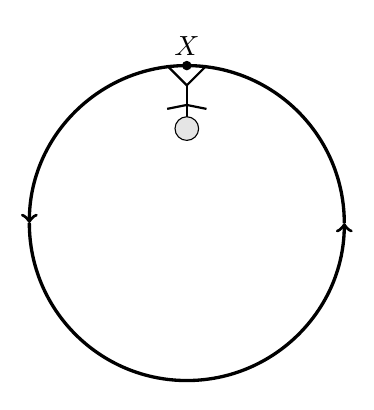
\begin{tikzpicture}
    %% Cirlce
    \draw[very thick,->] (-2,0) arc (180:360:2);
    \draw[very thick,->] (+2,0) arc (0:180:2);
    %% Point X
    \draw[fill] (0,2) circle (1.5pt) node[anchor=south] {$X$};
    %% Man In Box
    \begin{scope}[rotate=180,yshift=-2cm]
        \draw[thick] (0,0.25) -- (0,0.75);
        %% Legs
        \draw[thick] (0,0.25) -- (-0.25,0);
        \draw[thick] (0,0.25) -- (+0.25,0);
        %% Arms
        \draw[thick] (0,0.50) -- (-0.25,0.55);
        \draw[thick] (0,0.50) -- (+0.25,0.55);
        %% Head
        \draw[fill=white!90!black] (0,0.80) circle (0.15cm);
    \end{scope}
\end{tikzpicture}
}

\element{halliday-mc}{
\begin{question}{halliday-ch06-q62}
    A giant wheel, having a diameter of \SI{40}{\meter},
        is fitted with a cage and platform on which a man of mass $m$ stands. 
    The wheel is rotated in a vertical plane at such a speed that the force exerted by the man on the platform is equal to his weight when the cage is at $X$, as shown. 
    \begin{center}
        \hallidayChSixQSixtyTwo
    \end{center}
    The net force on the man at point $X$ is:
    \begin{multicols}{2}
    \begin{choices}
        \wrongchoice{zero}
        \wrongchoice{$mg$, down}
        \wrongchoice{$mg$, up}
      \correctchoice{$2mg$, down}
        \wrongchoice{$2mg$, up}
    \end{choices}
    \end{multicols}
\end{question}
}

\element{halliday-mc}{
\begin{question}{halliday-ch06-q63}
    A giant wheel, \SI{40}{\meter} in diameter,
        is fitted with a cage and platform on which a man can stand.
    The wheel rotates at such a speed that when the cage is at $X$
        (as shown) the force exerted by the man on the platform is equal to his weight. 
    \begin{center}
        \hallidayChSixQSixtyTwo
    \end{center}
    The speed of the man is:
    \begin{multicols}{3}
    \begin{choices}
        \wrongchoice{\SI{14}{\meter\per\second}}
      \correctchoice{\SI{20}{\meter\per\second}}
        \wrongchoice{\SI{28}{\meter\per\second}}
        \wrongchoice{\SI{80}{\meter\per\second}}
        \wrongchoice{\SI{120}{\meter\per\second}}
    \end{choices}
    \end{multicols}
\end{question}
}

\element{halliday-mc}{
\begin{question}{halliday-ch06-q64}
    A person riding a Ferris wheel is strapped into her seat by a seat belt. 
    The wheel is spun so that the centripetal acceleration is $g$.
    Select the correct combination of forces that act on her when she is at the top. 
    In the table $F_g$ = force of gravity, down;
        $F_b$ = seat belt force, down;
        and $F_s$ = seat force, up.
    \begin{center}
    \begin{tabu}{cX[c]X[c]X[c]}
        \toprule
        \#  & $F_g$ & $F_b$ & $F_s$ \\
        \midrule
        $A$ & 0     & $mg$  & 0 \\
        $B$ & $mg$  & 0     & 0 \\
        $C$ & 0     & 0     & $mg$ \\
        $D$ & $mg$  & $mg$  & 0 \\
        $E$ & $mg$  & 0     & $mg$ \\
        \bottomrule
    \end{tabu}
    \end{center}
    \begin{multicols}{5}
    \begin{choices}[o]
        \wrongchoice{$A$}
      \correctchoice{$B$}
        \wrongchoice{$C$}
        \wrongchoice{$D$}
        \wrongchoice{$E$}
    \end{choices}
    \end{multicols}
\end{question}
}

\element{halliday-mc}{
\begin{question}{halliday-ch06-q65}
    One end of a \SI{1.0}{\meter} long string is fixed, the other end is attached to a \SI{2.0}{\kilo\gram} stone. 
    The stone swings in a vertical circle,
        passing the bottom point at \SI{4.0}{\meter\per\second}.
    The tension force of the string at this point is about:
    \begin{multicols}{3}
    \begin{choices}
        \wrongchoice{zero}
        \wrongchoice{\SI{12}{\newton}}
        \wrongchoice{\SI{20}{\newton}}
        \wrongchoice{\SI{32}{\newton}}
      \correctchoice{\SI{52}{\newton}}
    \end{choices}
    \end{multicols}
\end{question}
}

\element{halliday-mc}{
\begin{question}{halliday-ch06-q66}
    One end of a \SI{1.0}{\meter} string is fixed,
        the other end is attached to a \SI{2.0}{\kilo\gram} stone. 
    The stone swings in a vertical circle,
        passing the top point at \SI{4.0}{\meter\per\second}. 
    The tension force of the string at this point is about:
    \begin{multicols}{3}
    \begin{choices}
        \wrongchoice{\SI{0}{\newton}}
      \correctchoice{\SI{12}{\newton}}
        \wrongchoice{\SI{20}{\newton}}
        \wrongchoice{\SI{32}{\newton}}
        \wrongchoice{\SI{52}{\newton}}
    \end{choices}
    \end{multicols}
\end{question}
}

\element{halliday-mc}{
\begin{question}{halliday-ch06-q67}
    A coin is placed on a horizontal phonograph turntable. 
    Let $N$ be the magnitude of the normal force exerted by the turntable on the coin,
        $f$ be the magnitude of the frictional force exerted by the turntable on the coin,
        and $f_{s,\text{max}}$ be the maximum possible force of static friction. 
    The speed of the turntable is increased in small steps. 
    If the coin does not slide, then:
    \begin{choices}
        \wrongchoice{$N$ increases, $f$ increases, and $f_{s,\text{max}}$ stays the same}
        %% NOTE: B is duplicate of E (sic)
        \wrongchoice{$N$ increases, $f$ increases, and $f_{s,\text{max}}$ increases}
      \correctchoice{$f$ increases and both $N$ and $f_{\text{s,max}}$ stay the same}
        \wrongchoice{$N$, $f$, and $f_{s,\text{max}}$ all stay the same}
        \wrongchoice{$N$, $f$, and $f_{s,\text{max}}$ all increase}
    \end{choices}
\end{question}
}

\element{halliday-mc}{
\begin{question}{halliday-ch06-q68}
    The iron ball shown is being swung in a vertical circle at the end of a \SI{0.7}{\meter} long string. 
    \begin{center}
    \begin{tikzpicture}
        \draw[dashed] (0,0) circle (2cm);
        \draw[fill] (45:2) circle (2pt);
        \draw[thick] (0,0) -- (45:2);
        \draw[thick,->] (35:2.3) arc(35:55:2.3);
    \end{tikzpicture}
    \end{center}
    How slowly can the ball go through its top position without having the string go slack?
    \begin{multicols}{3}
    \begin{choices}
        \wrongchoice{\SI{1.3}{\meter\per\second}}
      \correctchoice{\SI{2.6}{\meter\per\second}}
        \wrongchoice{\SI{3.9}{\meter\per\second}}
        \wrongchoice{\SI{6.9}{\meter\per\second}}
        \wrongchoice{\SI{9.8}{\meter\per\second}}
    \end{choices}
    \end{multicols}
\end{question}
}

\element{halliday-mc}{
\begin{question}{halliday-ch06-q69}
    A block is suspended by a rope from the ceiling of a car. 
    When the car rounds a \SI{45}{\meter} radius horizontal curve at \SI{22}{\meter\per\second} (about \SI{50}{\mile\per\hour}),
        what angle does the rope make with the vertical?
    \begin{multicols}{3}
    \begin{choices}
        \wrongchoice{\ang{0}}
        \wrongchoice{\ang{25}}
      \correctchoice{\ang{48}}
        \wrongchoice{\ang{65}}
        \wrongchoice{\ang{90}}
    \end{choices}
    \end{multicols}
\end{question}
}

\element{halliday-mc}{
\begin{question}{halliday-ch06-q70}
    Circular freeway entrance and exit ramps are commonly banked to handle a car moving at \SI{13}{\meter\per\second}. 
    To design a similar ramp for \SI{26}{\meter\per\second} one should:
    \begin{choices}
        \wrongchoice{increase radius by factor of $2$}
        \wrongchoice{decrease radius by factor of $2$}
      \correctchoice{increase radius by factor of $4$}
        \wrongchoice{decrease radius by factor of $\sqrt{4}$}
        \wrongchoice{increase radius by factor of $2$}
    \end{choices}
\end{question}
}

\element{halliday-mc}{
\begin{question}{halliday-ch06-q71}
    At what angle should the roadway on a curve with a \SI{50}{\meter}
        radius be banked to allow cars to negotiate the curve at
        \SI{12}{\meter\per\second} even if the roadway is icy
        (and the frictional force is zero)?
    \begin{multicols}{3}
    \begin{choices}
        \wrongchoice{\ang{0}}
      \correctchoice{\ang{16}}
        \wrongchoice{\ang{18}}
        \wrongchoice{\ang{35}}
        \wrongchoice{\ang{73}}
    \end{choices}
    \end{multicols}
\end{question}
}


\endinput


